\documentclass[11pt,a4paper]{article}
\usepackage{algorithm}
\usepackage{algpseudocode}
\usepackage{amsmath}
\usepackage[final]{pdfpages}
\usepackage{forest}
\usepackage{mathtools}
\DeclarePairedDelimiter\ceil{\lceil}{\rceil}
\DeclarePairedDelimiter\floor{\lfloor}{\rfloor}
\begin{document}
\author{Ankur Dhoot}
\title{CS 580 HW 2}
\maketitle

\section*{Q1}
We'll give an algorithm that runs in O(nlogr) time. 

Let S be the set of n numbers. Let K = {$k_{1}$, $k_{2}$, ... $k_{r}$} where 1 $\leq$ $k_{1}$ $<$ $k_{2}$ $<$ ... $<$ $k_{r}$ $\leq$ n. Let A[1...r] be an array where A[1] will store the $k_{1}st$ smallest number ... A[r] will store the $k_{r}th$ smallest number. 

We begin by finding the median element, x, of S and partitioning on x. This can be done in O(n) time as seen in CLRS 9.3. We denote the rank of the median as m. We then form the sets K1 and K2, where K1 contains the $k_{i}$ with $k_i$ $<$ m, and K2 contains the $k_i$ with $k_i$ $>$ m, except we subtract m from these $k_{i}$ since we'll be searching for the corresponding rank only in the right subarray of S. 

We then recursively call SELECT(S, lo, m-1, K1) to search in the left subarray for the elements whose ranks are in K1. Then, we call SELECT(S, m+1, hi, K2) to search in the right subarray for the elements whose ranks are in K2. In between, we check if the median element, x (with rank m), corresponded to a rank in K. If so, we append S[m] to A.

Note that the order of these calls insures that A has the property of being sorted with A[i] storing the $k_{i}th$ ranked element in S. 
\begin{algorithm}
	\caption{Select the k1, k2, .. kr(th) smallest elements in S}
	\begin{algorithmic}[1]
	\State Let A[1...r] be a global array to hold the elements
	\Function{SELECT}{S, lo, hi, K}
	\If{lo == hi}
		\State Append S[lo] to A
	\EndIf
	\State x = FIND-MEDIAN(S, lo, hi)  \Comment returns the index of the median
	\State exchange S[hi] with S[x]    \Comment put median as partition element
	\State PARTITION(S, lo, hi)        \Comment same method as in CLRS 7.1
	\State m = $\ceil*{\frac{hi - lo + 1}{2}}$  \Comment rank of median element in A[lo...hi]
	\State K1 = $\{$k $|$ k $\in$ K $\&$ k $<$ m$\}$ 
	\State K2 = $\{$(k - m) $|$ k $\in$ K $\&$ k $>$ m$\}$
	\If{size(K1) $\neq$ 0}
		\State SELECT(S, lo, m-1, K1)
	\EndIf
	\If{m $\in$ K} 
		\State Append S[m] to A
	\EndIf
	\If{size(K2) $\neq$ 0}
		\State SELECT(S, m+1, hi, K2)
	\EndIf
	\EndFunction
	\end{algorithmic}
	\end{algorithm}

Runtime: If we think about the recursion tree, the maximum number of nodes in a level is r which will occur at a depth of $\ceil*{logr}$. Reasoning: Take for example, r = 4. The maximum number of subproblems we can solve is r. Suppose, at some level, we are solving more than r subproblems. We only recurse on a subproblem if there remain ranks to be found in that subarray (i.e size(K1) $\neq$ 0 or size(K2) $\neq$ 0). Since K only has 4 ranks to be found, we can't be solving more than 4 subproblems at any level of the tree. Since we recurse on at most 2 subarrays, the maximum number of nodes will occur at $\ceil*{logr}$ depth. Thereafter, there will be a maximum of 4 nodes in a level, and we continually decrease each subproblem size by 2. The recursion tree for r = 4, in the worst case would look like:

\newpage

Since the first $\ceil*{logr}$ levels of the recursion tree each cost O(n) time independent of the subproblems, T(n) $\leq$ O(nlogr) + $\sum_{i=1}^{logn/r} \frac{n}{2^{i}r} r$ = O(nlogr) + $\sum_{i=1}^{logn/r} \frac{n}{2^{i}}$ O(nlogr) + O(n) = O(nlogr).

\begin{forest}
  for tree={
    draw,
    align=center
  }
  [n
    [n/2
      [n/4
      	[n/8
      		[n/16
      			[..]
      		]
      	]
      ]
      [n/4
      	[n/8
      		[n/16
      			[..]
      		]
      	]
      ]
    ]
    [n/2
      [n/4
      	[n/8
      		[n/16
      			[..]
      		]
      	]
      ]
      [n/4
      	[n/8
      		[n/16
      			[..]
      		]
      	]
      ]
    ]
  ]
\end{forest}

\newpage

\section*{Q2}
The algorithm for computing the minimum tri-distance amongst three points in P will be very similar to the algorithm given in CLRS 33.4, so we'll use the same notation. We presort X and Y as in CLRS 33.4 to avoid sorting the arrays in every subproblem. 

We partition the points into two sets $P_{L}$ and $P_{R}$ using the median x value. The three points with minimum tri-distance then all reside in $P_{L}$, all reside in $P_{R}$, or cross the partition. We recursively compute the tri-distance, $\delta_{1}$, among the points in $P_{L}$ and the tri-distance, $\delta_{2}$ among the points in $P_{R}$. We let $\delta$ = min($\delta_{1}$, $\delta_{2}$). 

We then create the array Y', which contains all points in the 2$\delta$ wide vertical strip centered on the median x value, same as in CLRS 33.4. We now compute the minimum tri-distance in the case that the points cross the partition. 

If the three points, ($p_{i}$, $p_{j}$, $p_{k}$), that comprise the minimum tri-distance cross the partition, it's clear that they must reside in a $\delta$ high rectangle in Y' (since trd($p_{i}$, $p_{j}$, $p_{k}$) $<$ $\delta$). The key insight is that for each point $p_{i}$ in Y', we need only check a constant number of ($p_{j}, p_{k}$) inside Y' to find the minimum tri-distance. 

If we divide a 2$\delta$ wide by $\delta$ high rectangle in Y' into 32 subrectangles of size $\delta$/4 x $\delta$/4, there can be at most 2 points in any subrectangle. Why? If we place three points as far as possible in any subrectangle (as shown below), then the tri-distance is $\delta$/4 + $\delta$/4 + $\sqrt{(\delta/4)^{2} + (\delta/4)^{2}}$ = $\delta$(1/2 + $\sqrt(2)$/4) $<$ $\delta$, a contradiction to how we defined $\delta$. Thus, there can be at most 2 points in any subrectangle. Thus, there can be at most 64 points in any 2$\delta$ x $\delta$ rectangle. 

Without loss of generality, suppose that $p_{i}$ is the lowest point of ($p_{i}$, $p_{j}$, $p_{k}$) (i.e $p_{i}$ precedes $p_{j}$ and $p_{k}$ in Y'). Then $p_{j}$ and $p_{k}$ must be among the 63 points following $p_{i}$. Thus, we need only check all $\binom{63}{2}$ possible pairs of points among the 63 points following $p_{i}$. 

Since $\binom{63}{2}$ is a constant, the recurrence relation is the same as in CLRS 33.4. That is, assuming we presort X and Y in O(nlogn) time, the recurrence is then T(n) = 2T(n/2) + O(n). At each step, we solve 2 subproblems of size n/2. Forming $P_{L}$, $P_{R}$, $X_{L}$, $X_{R}$, $Y_{L}$, $Y_{R}$, and Y' takes linear time as described in CLRS 33.4. For each point in Y', of which there are at most n, we need only do constant work to check $\binom{63}{2}$ tri-distances. Thus lines 10-12 run in O(n). Thus the recurrence gives us T(n) = O(nlogn). 

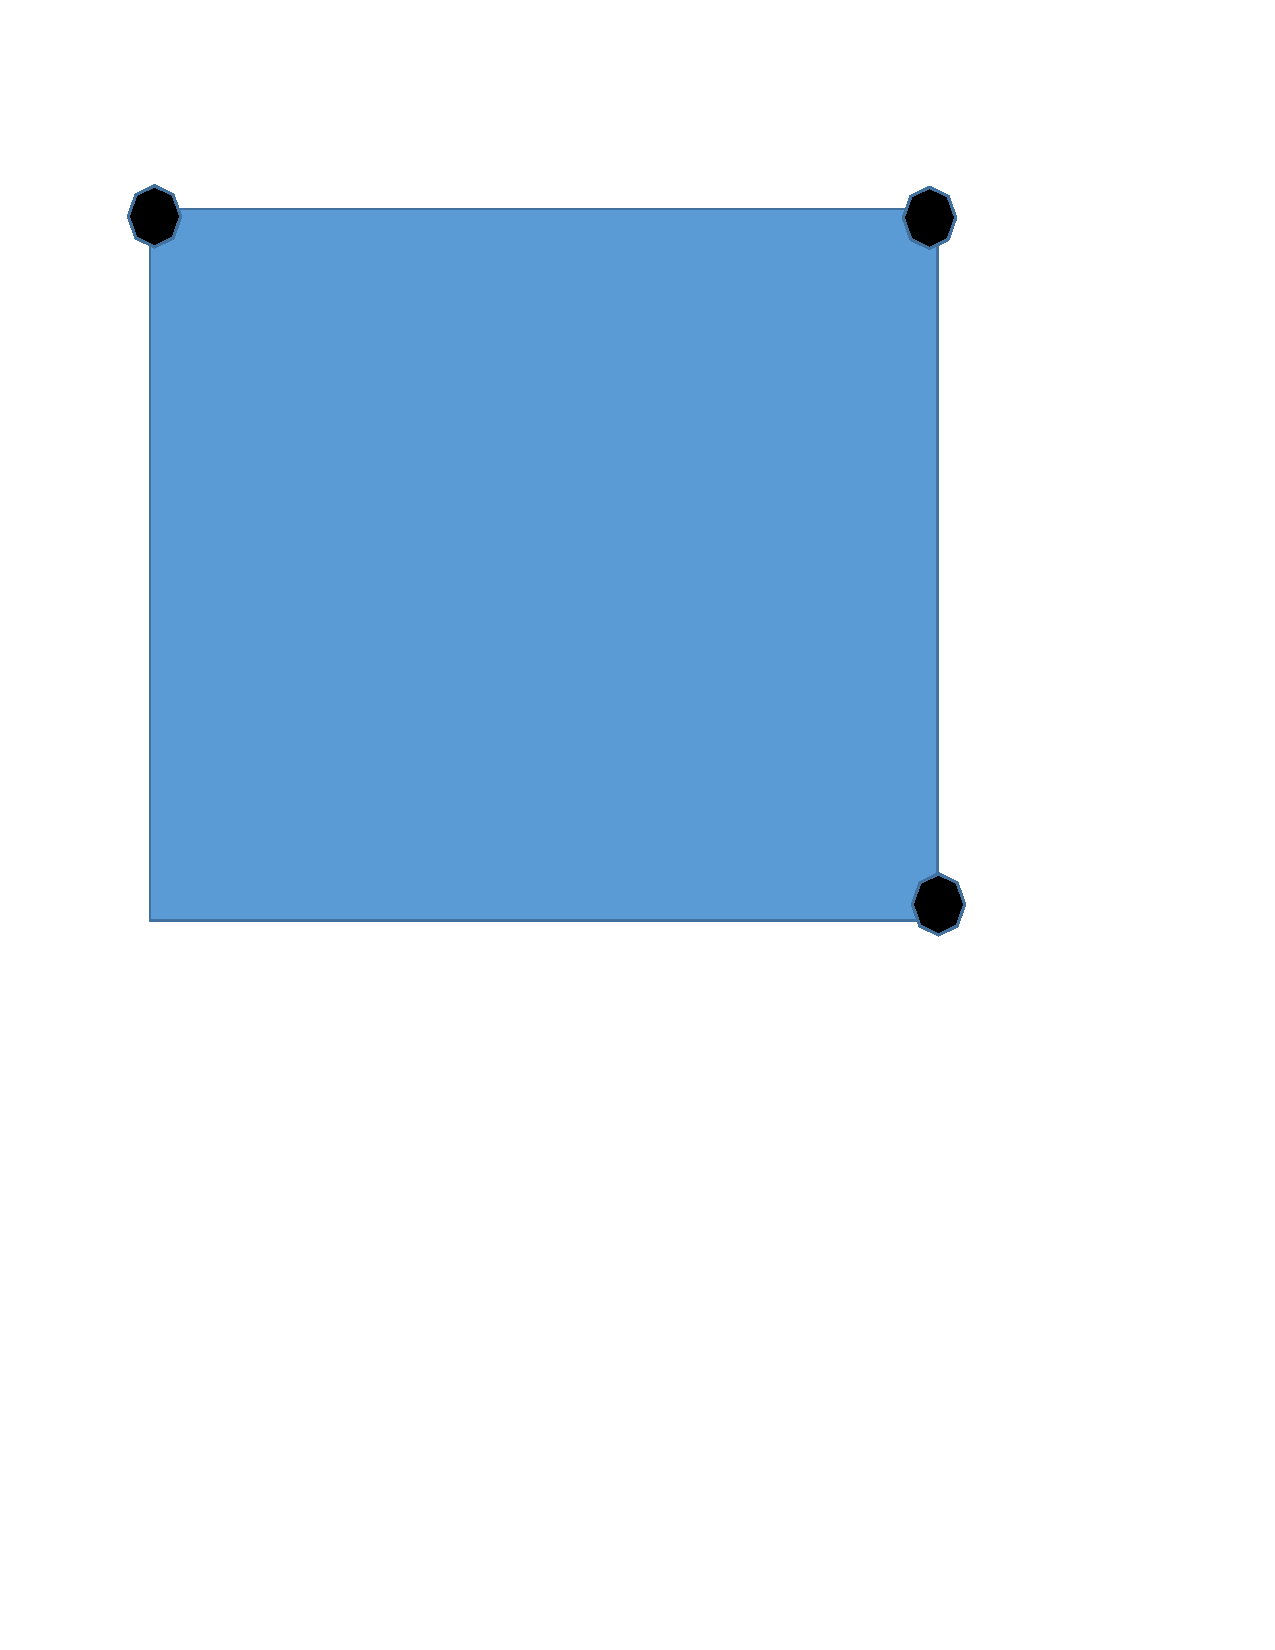
\includepdf[]{points.pdf}
\begin{algorithm}
	\caption{Find the three points whose pairwise distance sum is minimum among all sets of three points in P; X and Y are sorted by x and y coordinate, respectively}
	\begin{algorithmic}[1]
	\Function{TRIDISTANCE}{P, X, Y}
		\If{$|$P$|$ $<$ 6}
			\State Brute force all $\binom{P}{3}$ possibilities and \Return the min
		\EndIf
		\State Form $P_{L}$, $P_{R}$, $X_{L}$, $X_{R}$, $Y_{L}$, $Y_{R}$ as in CLRS 33.4
		\State $\delta_{1}$ = TRIDISTANCE($P_{L}$, $X_{L}$, $Y_{L}$)
		\State $\delta_{2}$ = TRIDISTANCE($P_{R}$, $X_{R}$, $Y_{R}$)
		\State $\delta$ = min($\delta_{1}$, $\delta_{2}$)
		\State Form array Y', the 2$\delta$ width strip as in CLRS 33.4
		\State For each point $p_{i}$ in Y', consider the next 63 points in Y'
		\State For each ($p_{j}$, $p_{k}$) in the $\binom{63}{2}$ pairs possible, compute trd($p_{i}$, $p_{j}$, $p_{k}$)
		\State Save the minimum as $\delta'$
		\State \Return min($\delta$, $\delta'$)
	\EndFunction
	\end{algorithmic}
	\end{algorithm}

\end{document}

